\documentclass[11pt]{beamer}
\usepackage{listings} % Include the listings-package
\usepackage[T1]{fontenc}
\usepackage[utf8]{inputenc}
\usepackage[english]{babel}
\usepackage{amsmath}
\usepackage{amssymb, amsfonts, latexsym, cancel}
\usepackage{float}
\usepackage{graphicx}
\usepackage{epstopdf}
\usepackage{subfigure}
\usepackage{hyperref}
%\usepackage{authblk}
\usepackage{blindtext}
\usepackage{booktabs} % Allows the use of \toprule, 
\usepackage{filecontents}
\usepackage{courier} %% Sets font for listing as Courier.
\usepackage{listings}
%\usepackage{listings, xcolor}
\lstset{
tabsize = 2, %% set tab space width
showstringspaces = false, %% prevent space marking in strings, string is defined as the text that is generally printed directly to the console
numbers = left, %% display line numbers on the left
commentstyle = \color{green}, %% set comment color
keywordstyle = \color{blue}, %% set keyword color
stringstyle = \color{red}, %% set string color
rulecolor = \color{black}, %% set frame color to avoid being affected by text color
basicstyle = \small \ttfamily , %% set listing font and size
breaklines = true, %% enable line breaking
numberstyle = \tiny,
}
\usepackage{caption}
\DeclareCaptionFont{white}{\color{white}}
\DeclareCaptionFormat{listing}{\colorbox{gray}{\parbox{\textwidth}{#1#2#3}}}
\captionsetup[lstlisting]{format=listing,labelfont=white,textfont=white}
\definecolor{urlColor}{rgb}{0.06, 0.3, 0.57}
\definecolor{linkColor}{rgb}{0.57, 0.0, 0.04}
\definecolor{fileColor}{rgb}{0.0, 0.26, 0.26}
\hypersetup{
    colorlinks=true,
    linkcolor=linkColor,
    filecolor=fileColor,      
    urlcolor=urlColor,
}
\urlstyle{same}
\setbeamercovered{transparent}

%\usetheme{Berkeley}
%\usetheme{Bergen}
\usetheme{Hannover}
%\usetheme{Malmoe}

\title[Expo IHC]{\Huge Interacción Humano Computador}
\subtitle{Donald A. Norman - 1983}
\author[Grupo 11]
{
	Luis Diego Valdivia Turpo  \\
	Alvaro Marcelo Zuñiga Cauna \\
	Michell Benjamin Pezo Centeno \\
	Karlo Jose Torres Aroquipa
}
\institute[UNSA]
{
Facultad de producción y servicios\\
Escuela de Ingeniería de Sistemas\\
Universidad Nacional de San Agustin - Arequipa
}

\date[2020-09-12]{\scriptsize{2020-09-12}}
%\logo{
\includegraphics[width=3.0cm]{img/logo_unsa.jpg}}
\titlegraphic{
\includegraphics[width=2.6cm]{img/logo_unsa.jpg}}

\begin{document}

\begin{frame}
\titlepage
\end{frame}

\begin{frame}
\frametitle{Indice}
\tableofcontents
\end{frame}

\section{Intro}
\begin{frame}
\frametitle{Intro}
\begin{itemize}
\item No deberia sorprendernos que las personas cometen errores al momento de usar sistemas informaticos.
\item En el trabajo de Norman se abordan reglas para mejorar esa situacion.
\end{itemize}
\end{frame}

\section{Lecciones}
\begin{frame}
\frametitle{Lecciones}
\begin{itemize}
\item Feedback.
\item Similitud de respuestas de secuencia.
\item Las acciones deben ser reversibles.
\item Consistencia del sistema.
\end{itemize}
\end{frame}


\section{Books}
\begin{frame}
\frametitle{Acciones reversibles}

{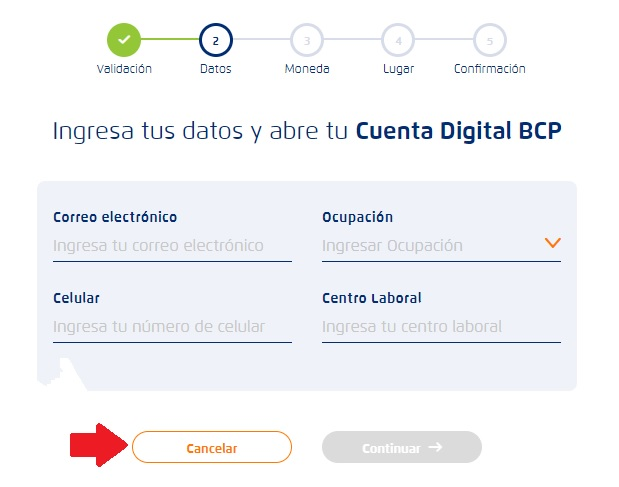
\includegraphics[width=10.0cm]{img/reversible.jpg}}

\end{frame}

\begin{frame}
\frametitle{Feedback}

{
\includegraphics[width=10.0cm]{img/feedback.jpg}}

\end{frame}

\begin{frame}
\frametitle{Similitud}

{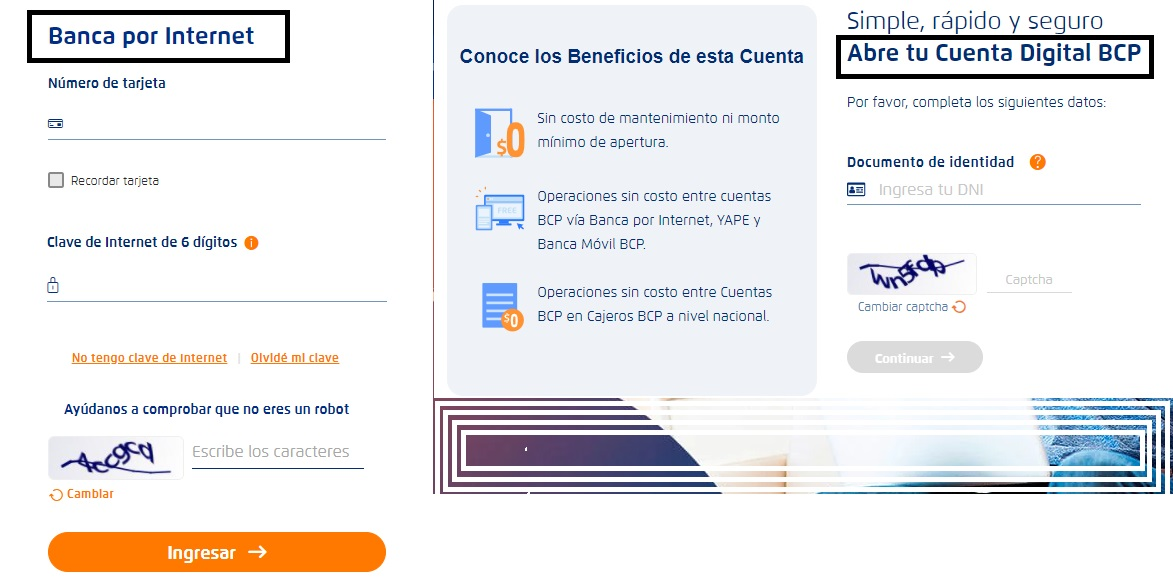
\includegraphics[width=10.0cm]{img/similitud.jpg}}

\end{frame}


\section{Referencias}
%References frame
\begin{frame}
\frametitle{Referencias}
\begin{itemize}
\item \href{https://www.researchgate.net/publication/220424605_Design_Rules_Based_on_Analyses_of_Human_Error}{Design Rules Based on Analyses of Human Error.}
\item \href{http://www.webnova.com.ar/los-cuatro-principios-del-buen-diseno-de-donald-norman/}{Cuatro Principios de un Buen Diseño-Norman}
\end{itemize}
\end{frame}

\end{document}